\documentclass[11pt]{exam}

\usepackage{amssymb, amsmath, amsthm, mathrsfs, multicol, graphicx}
\usepackage{tikz, pgfplots}


\def\d{\displaystyle}
\def\?{\reflectbox{?}}
\def\b#1{\mathbf{#1}}
\def\f#1{\mathfrak #1}
\def\c#1{\mathcal #1}
\def\s#1{\mathscr #1}
\def\r#1{\mathrm{#1}}
\def\N{\mathbb N}
\def\Z{\mathbb Z}
\def\Q{\mathbb Q}
\def\R{\mathbb R}
\def\C{\mathbb C}
\def\F{\mathbb F}
\def\A{\mathbb A}
\def\X{\mathbb X}
\def\E{\mathbb E}
\def\O{\mathbb O}
\def\pow{\mathscr P}
\def\inv{^{-1}}
\def\nrml{\triangleleft}
\def\st{:}
\def\~{\widetilde}
\def\rem{\mathcal R}
\def\iff{\leftrightarrow}
\def\Iff{\Leftrightarrow}
\def\and{\wedge}
\def\And{\bigwedge}
\def\AAnd{\d\bigwedge\mkern-18 mu\bigwedge}
\def\Vee{\bigvee}
\def\VVee{\d\Vee\mkern-18 mu\Vee}
\def\imp{\rightarrow}
\def\Imp{\Rightarrow}
\def\Fi{\Leftarrow}


\def\bar{\overline}

%\pointname{pts}
\pointsinmargin
\marginpointname{pts}
\marginbonuspointname{ bns pts}

\addpoints
\pagestyle{headandfoot}
%\printanswers

\def\target{(tbd)}
\header{MATH 131}{\bf\large Final Exam: Learning Target \target}{Fall 2025}
\runningfooter{}{}{}
\extrafootheight{-.45 in}



\begin{document}
\def\target{1}
%space for name
\noindent {\large\bf Name:} \underline{\hspace{2.5 in}}
\vskip 1em

\begin{questions}
  \question The height $s(t)$ of a model rocket (in feet) after $t$ seconds is given by the function with graph and table below.
  \begin{multicols}{2}

    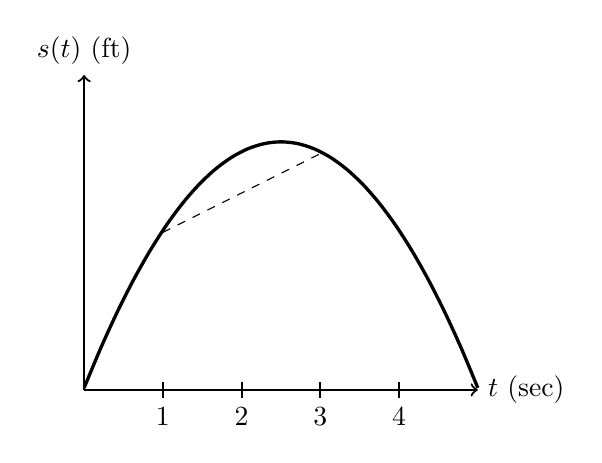
\begin{tikzpicture}
      % Axes:
      \draw[thick, ->] (0,0) -- (0,4) node[above] {$s(t)$ (ft)};
      \draw[thick, ->] (0,0) -- (5,0) node[right] {$t$ (sec)};
      \foreach \x in {1,2,3,4} \draw[thick] (\x,.1) -- (\x,-.1) node[below] {$\x$};
      \draw[very thick, domain=0:5] plot[smooth] (\x, {-.5*(\x-2.5)^2 + 3.15});
      \draw[dashed] (1,2) -- (3,3);
    \end{tikzpicture}

    \columnbreak
~
    \vfill

    \begin{tabular}{c|c}
      $t$ (sec) & $s(t)$ (ft) \\
      \hline
      0 & 0 \\
      1 & 25 \\
      2 & 40 \\
      3 & 40 \\
      4 & 25
    \end{tabular}
    \vfill
    \vfill
~
  \end{multicols}
  \begin{parts}
    \part Find the average velocity of the rocket between second 1 and second 3.
    \vfill
    \part Was the \emph{average} velocity of the rocket between second 1 and second 3 more than or less than the \emph{instantaneous} velocity at second 3?  Explain using either the graph or the table above.
    \vfill
  \end{parts}
\end{questions}

\newpage

\def\target{2}
%space for name
\noindent {\large\bf Name:} \underline{\hspace{2.5 in}}
\vskip 1em

\begin{questions}
  \question The graph of the function $f$ is given below.  

  \begin{center}
    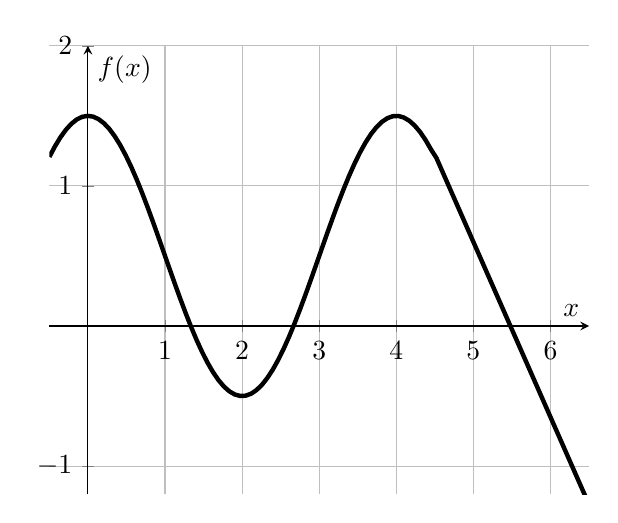
\begin{tikzpicture}[
      declare function={
        func(\x)= ( \x < 4.5) * (cos(deg(.5*pi*\x)) + .5) + (\x >= 4.5) * (-1.25*\x + 6.85);
      }
    ]
      \begin{axis}[
        axis x line=middle, axis y line=middle, ymin=-1.2, ymax=2, xmax=6.5, xlabel=$x$, ylabel=$f(x)$, grid=major
      ]
        \addplot [domain=-.5:6.5,samples=100, ultra thick]{func(x)};
      \end{axis}
    \end{tikzpicture}
  \end{center}


  \begin{parts}
    \part Use the graph to find $f'(5)$, the derivative of $f$ at $a=5$.  Show your work or explain why your answer is correct.
    \vfill
    \part Where is the derivative of $f$ largest between $x=0$ and $x = 6$?  That is, find a value of $a$ such that $f'(a)$ is as large as it is anywhere shown.  Explain why your answer is correct.
    \vfill
  \end{parts}


\end{questions}

\newpage

\def\target{3}
%space for name
\noindent {\large\bf Name:} \underline{\hspace{2.5 in}}
\vskip 1em
\begin{questions}
  \question Let $f(x) = x^2 + 5x + 2$.  Use the \emph{limit definition of the derivative} to find $f'(x)$, the derivative of $f$.  Show all your work.

  \vfill
\end{questions}


\newpage

\def\target{4}
%space for name
\noindent {\large\bf Name:} \underline{\hspace{2.5 in}}
\vskip 1em

\begin{questions}
  \question For each function graphed below, carefully sketch a graph of the functions derivative in the space provided below the original graph. 
  \begin{multicols}{2}
    % First function

        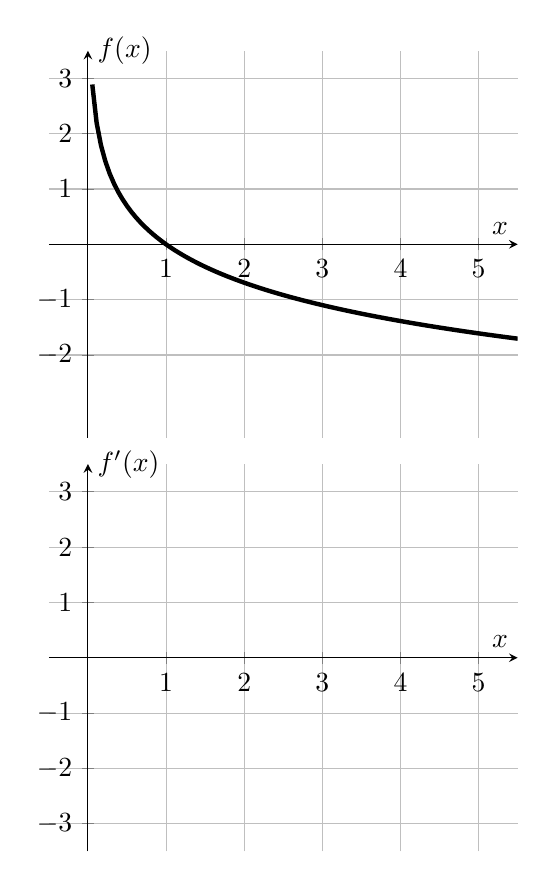
\begin{tikzpicture}[
      declare function={
        func(\x)= -ln(\x);
      }
    ]
      \begin{axis}[height=6.5cm,
        axis lines=center, ymin=-3.5, ymax=3.5, xmin=-0.5, xmax=5.5, xlabel=$x$, ylabel=$f(x)$, ylabel style={right}, ytick={-2,-1,...,4}, xtick={-4,-3,...,4,5}, grid=both
      ]
        \addplot [domain=0:5.5,samples=100, ultra thick]{func(x)};
      \end{axis}
        \begin{axis}[height=6.5cm, yshift=-5.25cm,
        axis lines=center, ymin=-3.5, ymax=3.5, xmin=-0.5, xmax=5.5, xlabel=$x$, ylabel=$f'(x)$, ylabel style={right}, ytick={-3,-2,-1,...,4}, xtick={-4,-3,...,4,5}, grid=both
      ]
      \end{axis}  

    \end{tikzpicture}
\vskip 1em
        % Second function
        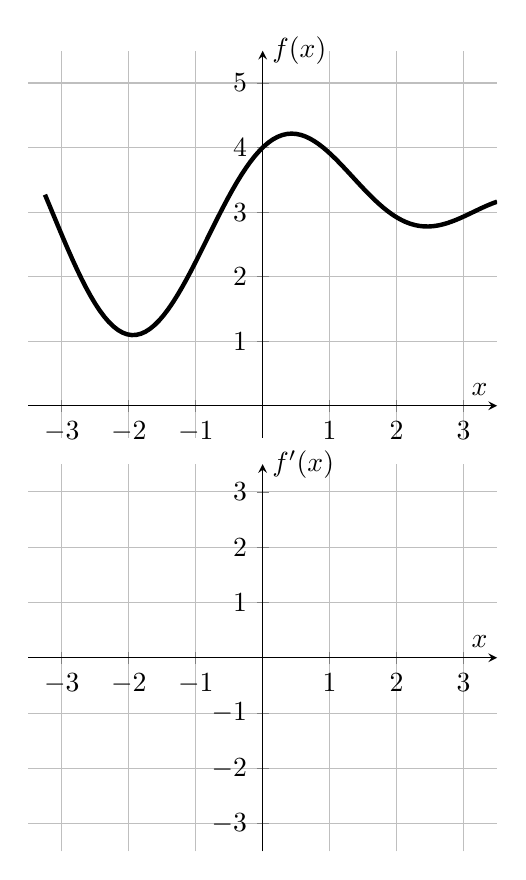
\begin{tikzpicture}[
      declare function={
        func(\x)= sin(deg(\x))+cos(deg(1.5*\x))+3;
      }
    ]
      \begin{axis}[height=6.5cm,
        axis lines=center, ymin=-0.5, ymax=5.5, xmin=-3.5, xmax=3.5, xlabel=$x$, ylabel=$f(x)$, ylabel style={right}, ytick={-2,-1,...,4,5}, xtick={-4,-3,...,4}, grid=both
      ]
        \addplot [domain=-3.25:3.5,samples=100, ultra thick]{func(x)};
      \end{axis}
      \begin{axis}[height=6.5cm, yshift=-5.25cm,
        axis lines=center, ymin=-3.5, ymax=3.5, xmin=-3.5, xmax=3.5, xlabel=$x$, ylabel=$f'(x)$, ylabel style={right}, ytick={-3,-2,-1,...,4}, xtick={-4,-3,...,4}, grid=both
      ]
      \end{axis}  

    \end{tikzpicture}
    

    \columnbreak

    % Third function

            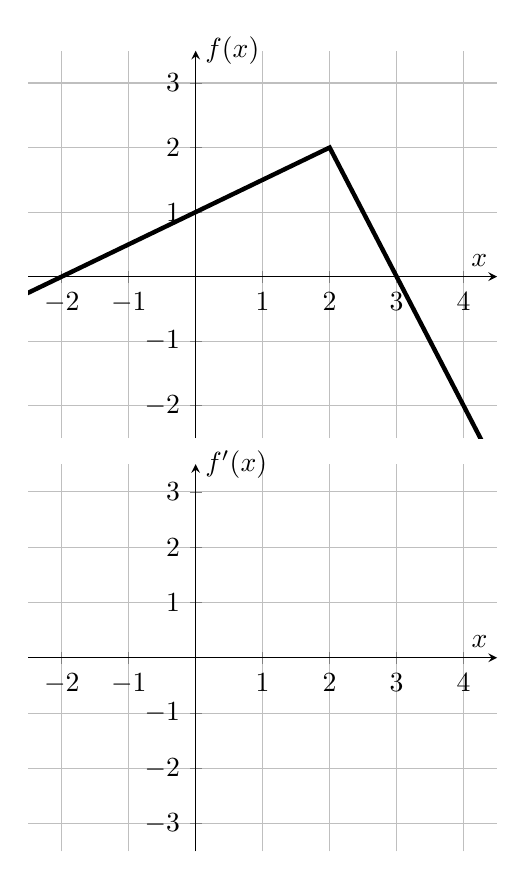
\begin{tikzpicture}[
      declare function={
        func(\x)= (.5*x + 1) * (x < 2) + (-2*x + 6) * (x >= 2) ;
      }
    ]
      \begin{axis}[height=6.5cm,
        axis lines=center, ymin=-2.5, ymax=3.5, xmin=-2.5, xmax=4.5, xlabel=$x$, ylabel=$f(x)$, ylabel style={right}, ytick={-2,-1,...,4}, xtick={-4,-3,...,4}, grid=both
      ]
        \addplot [domain=-3:4.5,samples=100, ultra thick]{func(x)};
      \end{axis}
        \begin{axis}[height=6.5cm, yshift=-5.25cm,
        axis lines=center, ymin=-3.5, ymax=3.5, xmin=-2.5, xmax=4.5, xlabel=$x$, ylabel=$f'(x)$, ylabel style={right}, ytick={-3,-2,-1,...,4}, xtick={-4,-3,...,4}, grid=both
      ]
      \end{axis}  
    \end{tikzpicture}

    
\vskip .5em
        
        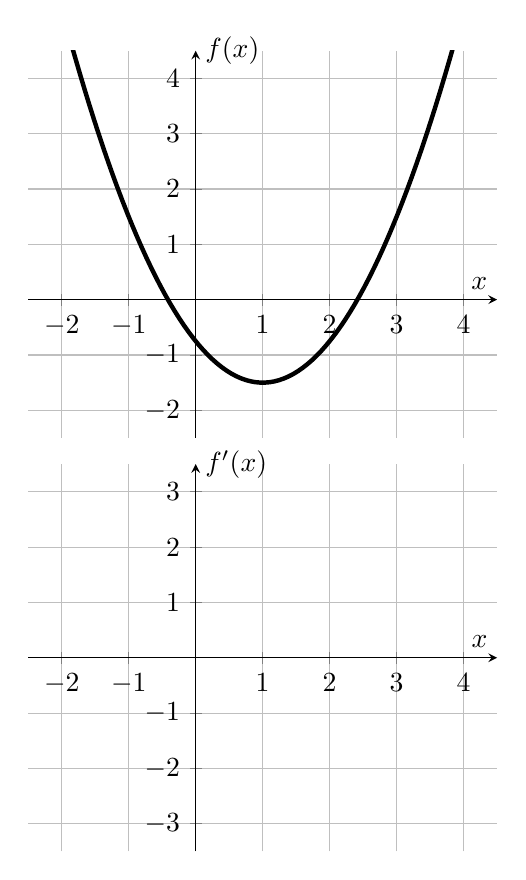
\begin{tikzpicture}[
      declare function={
        func(\x)= .75*( \x - 1)^2 - 1.5 ;
      }
    ]
      \begin{axis}[height=6.5cm,
        axis lines=center, ymin=-2.5, ymax=4.5, xmin=-2.5, xmax=4.5, xlabel=$x$, ylabel=$f(x)$, ylabel style={right}, ytick={-2,-1,...,4}, xtick={-4,-3,...,4}, grid=both
      ]
        \addplot [domain=-3:4,samples=100, ultra thick]{func(x)};
      \end{axis}
        \begin{axis}[height=6.5cm, yshift=-5.25cm,
        axis lines=center, ymin=-3.5, ymax=3.5, xmin=-2.5, xmax=4.5, xlabel=$x$, ylabel=$f'(x)$, ylabel style={right}, ytick={-3,-2,-1,...,4}, xtick={-4,-3,...,4}, grid=both
      ]
      \end{axis}  

    \end{tikzpicture}
    
  \end{multicols}
\end{questions}


\newpage

\def\target{5}
%space for name
\noindent {\large\bf Name:} \underline{\hspace{2.5 in}}
\vskip 1em
\begin{questions}
 \question The amount of food a carnivorous emu eats is a function of its age.  That is, $m(t)$ is the number of ounces of meat the emu will eat per day, $t$ weeks after it is born

Write sentences accurately interpreting the two equations below, \emph{including units}.  Your sentences must use all numbers in the equation.
\[
m(15) = 37 \qquad \qquad m'(15) = 3
\]

\vfill

\question The number of eggs a carnivorous emu produces each week is a function of the amount it eats.  That is, $g(m)$ is the number of eggs produced each week when an emu eats $m$ ounces of food each day.

Write a sentence accurately interpreting the two equations below, \emph{including units}.  Your sentence must use all numbers in the equation.
\[
g(37) = 3 \qquad\qquad g'(37) = 0.25
\]

\vfill
\end{questions}



\newpage

\def\target{6}
%space for name
\noindent {\large\bf Name:} \underline{\hspace{2.5 in}}
\vskip 1em


\begin{questions}
 \question The function $f$ is graphed below.  Use the graph to determine whether the first or second derivatives of $f$ are positive, negative, zero at the given points (circle the correct answer).  Justify your answer by filling in the blanks.

\begin{multicols}{2}
          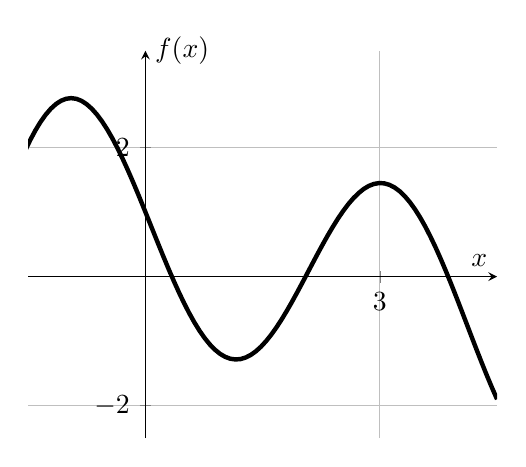
\begin{tikzpicture}[
      declare function={
        func(\x)= -2*sin(deg(1.5*\x)) + 1*cos(deg(.7*\x));
      }
    ]
      \begin{axis}[height=6.5cm,
        axis lines=center, ymin=-2.5, ymax=3.5, xmin=-1.5, xmax=4.5, xlabel=$x$, ylabel=$f(x)$, ylabel style={right}, ytick={}, xtick={3}, grid=major
      ]
        \addplot [domain=-2:4.5,samples=100, ultra thick]{func(x)};
      \end{axis}

    \end{tikzpicture}

    \columnbreak
    $f'(0)$ is: positive / negative / zero 
    \vskip 1ex
    because near $x=0$, $f(x)$ is \underline{\hspace{1in}} 
    \vskip 1.5ex
    $f''(0)$ is: positive / negative / zero 
    \vskip 1ex
    because near $x=0$, $f(x)$ is \underline{\hspace{1in}} 
    \vskip 1.5ex

    $f'(3)$ is: positive / negative / zero 
    \vskip 1.5ex
    because near $x=3$, $f(x)$ is \underline{\hspace{1in}} 

\vskip 1.5ex

    $f''(3)$ is: positive / negative / zero
    \vskip 1ex
    because near $x=3$, $f(x)$ is \underline{\hspace{1in}} 
  \end{multicols}

\question The function $g$ has a \textbf{derivative} $g'$ with values given in the following table.  Circle the characteristics of $g$, $g'$, and $g''$ that you can conclude from the table at the specified point.

\begin{center}
\begin{tabular}{c|ccccc}
$x$     & 0 & 1 & 2 & 3 & 4 \\ \hline
$g'(x)$ & -1 & 1 & 3  & 6  & 10
\end{tabular}
\end{center}


\begin{parts}
\part What can you conclude about $g'(2)$?
\vfill
$g'(2)$ is: positive / negative / zero / sign can't be determined.
\vfill
$g'(2)$ is: increasing / decreasing / flat / direction can't be determined.

\vfill
\part What can you say about $g''(2)$?  
\vfill
$g''(2)$ is: positive / negative / zero / sign can't be determined.

\vfill
\part What can you say about $g(2)$, the original function whose derivative is given in the table?
\vfill

$g(2)$ is: concave up / concave down / linear / shape can't be determined.
\vfill
$g(2)$ is: increasing / decreasing / flat / direction can't be determined.
\vfill
$g(2)$ is: positive / negative / zero / sign can't be determined.
\end{parts}

\end{questions}


\newpage

\def\target{7}
%space for name
\noindent {\large\bf Name:} \underline{\hspace{2.5 in}}
\vskip 1em
\begin{questions}
  \question Suppose you know that the function $f$ passes through the point $(1,5)$ and has first derivative
\[
f'(x) = 3^x.
\]
\begin{parts}
\part Find the equation of the tangent line to the the function $f(x)$ at the point $(1,5)$.
\vfill
\vfill
\part Use the tangent line (or the equivalent \emph{local linearization}) to approximate $f(0.9)$.  Show your work.
\vfill
\part Suppose you found out that $f''(1) = 3.3$.  What does this tell you about the shape of $f$ near $x = 1$?  Does this mean your approximation for $f(0.9)$ is an over estimate or under estimate?  Briefly explain.
\vfill
\end{parts}
\end{questions}

\newpage

\def\target{8}
%space for name
\noindent {\large\bf Name:} \underline{\hspace{2.5 in}}
\vskip 1em

For each function given below, find its derivative (using basic derivative rules).
\begin{questions}

\question $f(x) = 2 + 3x +4x^5$
\vfill
\question $f(x) = 3^x - e^x + 3^e$
\vfill
\question $f(x) = 2\cos(x) - 3\sin(x)$
\vfill
\question $f(x) = \d\frac{3}{x^2} - \sqrt[5]{x}$
\vfill
\end{questions}

\newpage

\def\target{9}
%space for name
\noindent {\large\bf Name:} \underline{\hspace{2.5 in}}
\vskip 1em
Find the derivatives of the following functions, using the product and quotient rules as appropriate.
\begin{questions}

  \question $f(x) = \cos(x)x^{-2}$
  \vfill
  \question $f(x) = \dfrac{e^x + 5}{x^2 + 1}$
  \vfill
  \question $f(x) = x^3\sin(x)(x^5 - 2)$
  \vfill
  
\end{questions}

\newpage

\def\target{10}
%space for name
\noindent {\large\bf Name:} \underline{\hspace{2.5 in}}
\vskip 1em
Find the derivatives of the following functions, using the chain rule.
\begin{questions}
\question $f(x) = \cos(5^x)$

\vfill

\question $f(x) = \sqrt{x^3 + 2x}$

\vfill

\question $f(x) = e^{\sin(\ln(x))+2}$

\vfill
\end{questions}

\newpage

\def\target{11}
%space for name
\noindent {\large\bf Name:} \underline{\hspace{2.5 in}}
\vskip 1em
Find the derivatives of the following functions.  You will need to use a combination of multiple rules.
\begin{questions}
  \question $f(x) = \d\cos\left(\frac{x^4+2}{x^7+1}\right)$
  \vfill
  \question $f(x) = 3^{x^2+1}\ln(x^3+4)$ 
\vfill
\end{questions}

\newpage

\def\target{12}
%space for name
\noindent {\large\bf Name:} \underline{\hspace{2.5 in}}
\vskip 1em

\begin{questions}
 \question Consider the curve defined implicitly by 
 \[
  x^2 - xy = 5y - y^2.
 \]
 \begin{parts}
 \part Use implicit differentiation to find $\dfrac{dy}{dx}$.  Show your work.
 \vfill
 \vfill
 \part Find the slope of the line tangent to the curve at the point $(0,5)$.
 \vfill
 \end{parts}
\end{questions}

\newpage

\def\target{13}
%space for name
\noindent {\large\bf Name:} \underline{\hspace{2.5 in}}
\vskip 1em
\begin{questions}
\question A mommy emu is out foraging due north of her next when her baby takes off running away from the nest due east.  By the time the baby emu is 30 feet away from the nest, it is running at 10 feet per second.  At this time, the mom is 40 feet from the nest, running due south at 15 feet per second (directly towards the nest, because emu's don't understand diagonal shortcuts).  

At what rate is the (diagonal) distance between the baby and momma decreasing at this instant?
\end{questions}


\newpage

\def\target{14}
%space for name
\noindent {\large\bf Name:} \underline{\hspace{2.5 in}}
\vskip 1em
You want to build a new habitat for your emus so they don't run away.  You must enclose a rectangular fields with fence, plus also add a fence separating the field into two equal sized rectangles.  If you have 500 feet of fence, what is the largest habitat you can construct?  Show all your work.


\newpage

\def\target{15}
%space for name
\noindent {\large\bf Name:} \underline{\hspace{2.5 in}}
\vskip 1em
\begin{questions}
\question The function $f(x)$ (which you don't know) has \emph{first and second derivatives}
\[
f'(x) = x(x+3)(x-2)
\]
\[
f''(x) = 3 x^2 + 2x - 6
\]
Using these provided derivatives, find all \underline{critical numbers} of the original function $f(x)$, and then use the first or second derivative tests to classify them as local maximums, local minimums, or neither.  Then give the intervals on which $f$ is increasing or decreasing.  

Use the middle of the page to show your work and record your answers at the bottom of the page.
\vfill
Critical numbers:
\vskip 1em
Local maximum(s) at $x = $
\vskip 1em
Local minimum(s) at $x = $
\vskip 1em
$f$ is increasing on the interval(s):
\vskip 1em
$f$ is decreasing on the interval(s):
\end{questions}


\newpage

\def\target{16}
%space for name
\noindent {\large\bf Name:} \underline{\hspace{2.5 in}}
\vskip 1em

\begin{questions}
\question Find the limit, using L'H\^opital's rule if appropriate:
\[
\lim_{x \to 1}\frac{x^2 + x - 2}{7x^2 - 4x - 3}
\]
\vfill
\question Evaluate the limit at infinity, using L'H\^opital's rule if appropriate:
\[
\lim_{x \to \infty}\frac{15x+12}{3e^x - 100}
\]
\vfill
\end{questions}


\newpage

\def\target{17}
%space for name
\noindent {\large\bf Name:} \underline{\hspace{2.5 in}}
\vskip 1em
\begin{questions}
\question The \emph{velocity} $v(t)$, in feet per second, of a model rocket, $t$ seconds after launch, has graph shown below.  

\begin{center}
    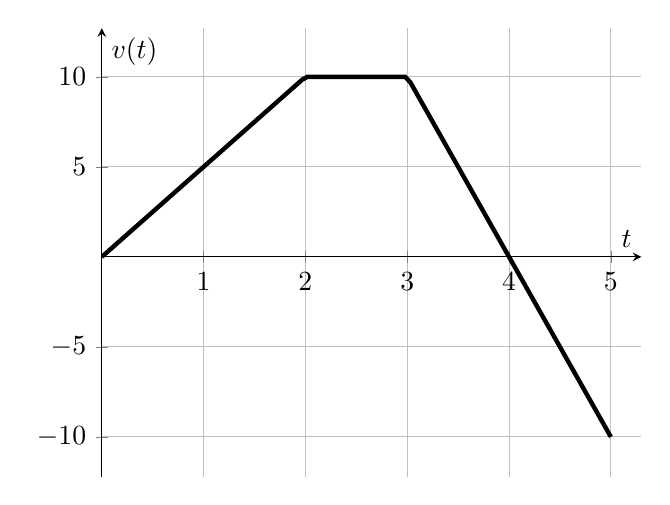
\begin{tikzpicture}[
      declare function={
        func(\x) = ( \x < 2) * (5*\x) + and(\x >= 2, \x < 3) * (10) + (\x >= 3)*((-10*\x)+40);
      }
    ]
      \begin{axis}[
        axis x line=middle, axis y line=middle, ymin=-12.2, ymax=12.7, xmin=0, xmax=5.3, xlabel=$t$, ylabel=$v(t)$, grid=major
      ]
        \addplot [domain=0:5, samples=100, ultra thick]{func(x)};
      \end{axis}
    \end{tikzpicture}
\end{center}
\begin{parts}
\part Find the total distance traveled by the rocket in the first four seconds (between seconds 0 and 4).  Briefly explain how you found your answer.
\vfill
\part Find the total \emph{change in position} of the rocket in the first \emph{five} seconds (between seconds 0 and 5).  Explain why this is less than the distance traveled in the first four seconds.
\vfill
\end{parts}
\end{questions}


\newpage

\def\target{18}
%space for name
\noindent {\large\bf Name:} \underline{\hspace{2.5 in}}
\vskip 1em

\begin{questions}
\question Consider the function $f(x) = (x-1)^2 + 1$.  Compute the left and right Riemann sums for $f(x)$ with $n = 4$ sub-intervals on the interval $[1,3]$.  Sketch the rectangles whose area represent the \emph{left} Riemann sum on the graph of $f$ below.

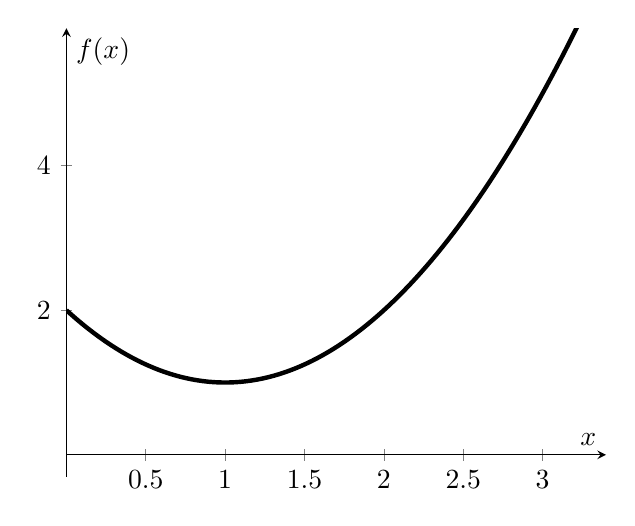
\begin{tikzpicture}[
      declare function={
        func(\x) = (\x - 1)^2 + 1;
      }
    ]
      \begin{axis}[
        axis x line=middle, axis y line=middle, ymin=-0.3, ymax=5.9, xmin=0, xmax=3.4, xlabel=$x$, ylabel=$f(x)$, grid=none
      ]
        \addplot [domain=0:3.4, samples=100, ultra thick]{func(x)};
      \end{axis}
    \end{tikzpicture}
    Left Riemann sum:
    \vfill
Right Riemann sum:
\vfill
\vskip 2em
\question If the function $f(x)$ above represents the \emph{rate of change} in height of your pet emu, in inches per week, $x$ weeks after you adopted him, what do the sums you computed above represent?
\vfill
\vfill
\end{questions}


\newpage

\def\target{19}
%space for name
\noindent {\large\bf Name:} \underline{\hspace{2.5 in}}
\vskip 1em

\begin{questions}
\question Consider the function $f(x)$ graphed below.  Assume each portion of the graph is either part of a line or part of a circle.

\begin{center}
    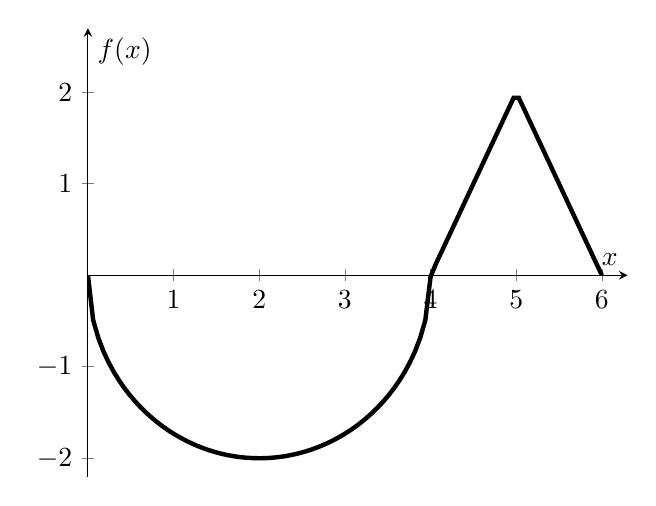
\begin{tikzpicture}[
      declare function={
        func(\x) = (\x <= 4)*(-sqrt(4-(\x-2)^2)) + and(\x > 4, \x <= 6) * (-2*abs(\x - 5)+2);
      }
    ]
      \begin{axis}[
        axis x line=middle, axis y line=middle, ymin=-2.2, ymax=2.7, xmin=0, xmax=6.3, xlabel=$x$, ylabel=$f(x)$, grid=none
      ]
        \addplot [domain=0:6, samples=100, ultra thick]{func(x)};
      \end{axis}
    \end{tikzpicture}
\end{center}
\begin{parts}
\part Give the exact value of $\int_0^6 f(x)\, dx$.  Briefly explain your answer.
\vfill
\part Find the total area between the curve and the $x$-axis (from 0 to 6).  What sum of integrals describes this (positive) area?
\vfill
\end{parts}
\end{questions}


\newpage

\def\target{20}
%space for name
\noindent {\large\bf Name:} \underline{\hspace{2.5 in}}
\vskip 1em

\begin{questions}
\question Consider the function \[f(x) = x^2 + 2x + 5.\]
Find the antiderivative $F(x)$ of $f(x)$.  Then check you work by computing $F'(x)$.
\vfill
\question Use your answer to the previous question to find the exact value of the definite integral:
\[
\int_1^3 x^2 + 2x + 5 \, dx.
\]
\vfill
\end{questions}

\end{document}
